
\section{牛顿环}

\begin{conclusion}[牛顿环]
\textbf{牛顿环}由一块平板玻璃和一枚曲率半径 \(R\) 很大的平凸透镜组成。两者之间形成一层厚度随半径变化的空气膜，相同厚度对应同一光程差，所以图样是同心圆环。

设距接触点半径为 \(r\) 处膜厚为 \(d\)。由几何关系
\[
r^2=R^2-(R-d)^2=2dR-d^2\approx 2dR\qquad(R\gg d),
\]
得
\[
d\approx \frac{r^2}{2R}.
\]
在反射光中，空气膜上下表面反射光之间有一次半波损失，因此
\[
\delta=2d+\frac{\lambda}{2}.
\]
于是反射暗环、明环分别满足
\[
\begin{cases}
2d=k\lambda, & \text{暗环},\quad k=0,1,2,\dots,\\[4pt]
2d=(2k-1)\dfrac{\lambda}{2}, & \text{明环},\quad k=1,2,3,\dots.
\end{cases}
\]
代入 \(d\approx r^2/(2R)\) 得
\[
r_k=\sqrt{kR\lambda}\quad(\text{暗环},\,k=0,1,2,\dots),\qquad
r_k=\sqrt{\frac{(2k-1)R\lambda}{2}}\quad(\text{明环},\,k=1,2,3,\dots).
\]
从反射光看，中心是暗点；从透射光看，中心是亮点。

又有
\[
r_k^2=R\left(k-\frac12\right)\lambda,\qquad
r_{k+1}^2-r_k^2=R\lambda,\qquad
r_{k+1}-r_k=\frac{R\lambda}{r_{k+1}+r_k},
\]
所以环纹间距随 \(r\) 增大而减小，图样呈现“中间疏，边缘密”。

牛顿环常见于以下几类问题：
\begin{enumerate}
  \item \textbf{检查平凸透镜曲率半径是否合格。} 受检元件与标准平板嵌合良好时，没有牛顿环，说明合格；若 \(R<R_0\)，加压时条纹向边缘移动；若 \(R>R_0\)，加压时条纹向中心移动。
  \item \textbf{测量透镜曲率半径。} 若测得第 \(k\) 个暗环半径为 \(r_k\)，第 \(k+m\) 个暗环半径为 \(r_{k+m}\)，则
  \[
  R=\frac{r_{k+m}^2-r_k^2}{m\lambda}.
  \]
  例如 \(\lambda=\SI{633}{nm}\)，\(r_k=\SI{5.63}{mm}\)，\(r_{k+5}=\SI{7.96}{mm}\)，得 \(R\approx\SI{10.0}{m}\)。
  \item \textbf{观察圆形油膜的干涉。} 若平面玻璃片上有一层圆形油膜，并从反射光中观察同心圆条纹，则仍可用牛顿环思路处理。以 \(\lambda=\SI{600}{nm}\)、\(n_1=1.50\)、\(n_2=1.20\) 为例，反射中的两次半波损失相互抵消，故
  \[
  \delta=2n_2d_k,\qquad d_k=k\frac{\lambda}{2n_2}=k\times\SI{250}{nm}\quad(k=0,1,2,\dots).
  \]
  因而油膜边缘 \(d_0=0\) 为明纹；当中心最高点与玻璃片上表面的距离 \(h=\SI{8.0e2}{nm}\) 时，可见 \(k=0,1,2,3\) 四条明纹。油膜展开时厚度减小，条纹数减少，条纹间距变大。
\end{enumerate}
\end{conclusion}




\begin{exercise}[牛顿环测曲率半径]
在牛顿环实验中，已知单色光波长为 \(\lambda\)，测得第 \(k\) 个暗环半径为 \(r_k\)，第 \(k+m\) 个暗环半径为 \(r_{k+m}\)。求平凸透镜的曲率半径 \(R\)。
\end{exercise}

\begin{solution}
题目给的是两个\textbf{暗环半径}，目标是求曲率半径 \(R\)。由反射暗环关系分别写出两级半径，再相减消去未知级次 \(k\)，于是
\[
\begin{aligned}
r_k^2&=kR\lambda,\qquad r_{k+m}^2=(k+m)R\lambda,\\
r_{k+m}^2-r_k^2&=(k+m)R\lambda-kR\lambda=mR\lambda
\implies
R=\frac{r_{k+m}^2-r_k^2}{m\lambda}.
\end{aligned}
\]
\(r^2/\lambda\) 的量纲是长度，和 \(R\) 一致。用平方差而不用半径直接相减的好处，是不必纠缠中心究竟记作第零级还是第一级；只要两条都是暗环，同一条公式就成立。
\end{solution}

\begin{exercise}[空气换成液体后牛顿环半径怎样反推折射率]
平凸透镜顶点和平板玻璃接触，用单色光垂直照射，观察反射光形成的牛顿环。测得中央暗斑外第 \(k\) 个暗环在空气中半径为 \(r_1\)。若将透镜和玻璃板之间的空气换成某种液体，且液体折射率小于玻璃折射率，第 \(k\) 个暗环半径变为 \(r_2\)。求该液体折射率。
\end{exercise}

\begin{solution}
同一个第 \(k\) 个暗环，对应的是同一级干涉条件；换液体后改变的是薄膜折射率，几何关系 \(d\approx r^2/(2R)\) 不变。

反射暗环条件可写成 \(2nd=k\lambda\)，又有 \(d=r^2/(2R)\)。空气中 \(n\approx1\)，所以
 \(2\cdot 1\cdot \frac{r_1^2}{2R}=k\lambda \implies r_1^2=kR\lambda.\) 
换成液体后，
 \(2n\frac{r_2^2}{2R}=k\lambda \implies nr_2^2=kR\lambda.\) 
两式相除得
 \(n=\frac{r_1^2}{r_2^2}.\) 
液体折射率 \(n>1\) 时，同一级暗环需要更小几何厚度，因此 \(r_2<r_1\)，于是 \(r_1^2/r_2^2>1\)，方向合理。牛顿环公式天然是半径平方关系，不能直接拿半径比来代替平方比。
\end{solution}

\begin{exercise}[2011级期末：浸入液体的牛顿环中心暗斑]
平凸透镜与平板玻璃构成牛顿环装置，整个装置浸入折射率为 \(n=\num{1.60}\) 的液体中。平凸透镜折射率为 \(\num{1.68}\)，平板玻璃折射率为 \(\num{1.58}\)。凸透镜可沿轴线 \(OO'\) 上下移动，用波长 \(\lambda=\SI{500}{nm}\) 的单色光垂直入射，从上方观察反射光。若调节后看到中心为暗斑，求凸透镜顶点到平板玻璃的最小距离。

\begin{center}
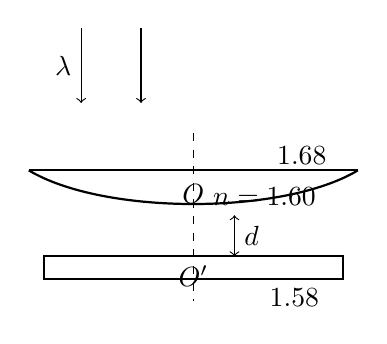
\begin{tikzpicture}[scale=0.95]
 \draw[->] (-1.5,2.6) -- (-1.5,1.6) node[midway,left] {\(\lambda\)};
 \draw[->] (-0.7,2.6) -- (-0.7,1.6);
 \draw[thick] (-2.2,0.7) .. controls (-1.2,0.1) and (1.2,0.1) .. (2.2,0.7);
 \draw[thick] (-2.2,0.7) -- (2.2,0.7);
 \draw[thick] (-2.0,-0.45) rectangle (2.0,-0.75);
 \draw[dashed] (0,1.2) -- (0,-1.05);
 \draw[<->] (0.55,0.10) -- (0.55,-0.45) node[midway,right] {\(d\)};
 \node at (0.95,0.35) {\(n=1.60\)};
 \node at (1.45,0.9) {\(1.68\)};
 \node at (1.35,-1.0) {\(1.58\)};
 \node[above] at (0,0.12) {\(O\)};
 \node[below] at (0,-0.45) {\(O'\)};
\end{tikzpicture}
\end{center}
\end{exercise}

\begin{solution}
液体膜内往返光程差需满足
 \(2nd=\left(k+\frac12\right)\lambda,\qquad k=0,1,2,\dots\) 
求最小距离，取 \(k=0\)，得
 \(d_{\min}=\frac{\lambda}{4n} =\frac{\SI{500}{nm}}{4\times1.60} =\SI{78.125}{nm}.\) 
因此最小距离约为 \(\SI{78.1}{nm}\)。如果中心两面相接 \(d=0\)，因为两次反射都没有相对半波损失，中心应为亮而不是暗；只凭“牛顿环中心常暗”直接选 \(0\)，就忽略了三种介质的折射率顺序。
\end{solution}


\begin{exercise}[两种波长第五个牛顿环明环对应膜厚差]
平凸透镜凸面朝下放在平玻璃板上，透镜刚好与玻璃板接触。波长分别为 \(\lambda_1=\SI{600}{nm}\)、\(\lambda_2=\SI{500}{nm}\) 的两种单色光垂直入射，观察反射光形成的牛顿环。求从中心向外数的两种光的第五个明环所对应的空气膜厚度之差。
\end{exercise}

\begin{solution}
反射牛顿环中心为暗，明环条件要带半级差。题目问的是膜厚差，不需要再把膜厚换成半径。

反射明环满足
 \(2d=\left(k-\frac12\right)\lambda,\qquad k=1,2,3,\dots\) 
第五个明环对应 \(k=5\)，故
 \(d=\frac{k-\frac12}{2}\lambda =\frac{9}{4}\lambda,\qquad \Delta d=\frac94(\lambda_1-\lambda_2) =\frac94(600-500)\,\si{nm} =\SI{225}{nm}.\) 
第五个明环不是 \(2d=5\lambda\)，而是 \(2d=(5-\frac12)\lambda\)。中心暗点会把明环条件整体错开半级。
\end{solution}

\begin{exercise}[2005级期末：迈克耳孙干涉仪中插入薄膜的厚度]
在迈克耳孙干涉仪的一支光路中，放入一片折射率为 \(n\) 的透明介质薄膜后，测出两束光的光程差改变量为一个波长 \(\lambda\)。求薄膜厚度。
\end{exercise}

\begin{solution}
迈克耳孙干涉仪中一支光路要往返一次。插入薄膜后，空气段被介质段替代，单程附加光程为 \((n-1)d\)，往返后要乘 \(2\)。

题目给出光程差改变量为一个波长满足
 \(2(n-1)d=\lambda \implies d=\frac{\lambda}{2(n-1)}.\) 
最容易漏掉的是迈克耳孙装置的往返程，把附加光程误写成 \((n-1)d\)。这里的 \(n-1\) 也说明我们比较的是“介质替代空气”带来的附加光程，而不是单纯的 \(nd\)。
\end{solution}

\begin{exercise}[2005级期末：牛顿环透镜上移时移过固定点的条纹数]
用波长为 \(\lambda\) 的单色光垂直照射牛顿环装置，观察从空气膜上下表面反射的光形成的牛顿环。若使平凸透镜从顶点与平面玻璃接触开始，慢慢垂直向上移动到两者距离为 \(d\)，求移过视场中某固定观察点的条纹数目。
\end{exercise}

\begin{solution}
固定观察点处的条纹变化，本质上是该点空气膜厚度随透镜整体上移而增加。反射牛顿环中，相邻同类条纹对应的膜厚变化为 \(\lambda/2\)。
透镜整体上移 \(d\) 后，固定观察点处空气膜厚度增加 \(d\)，所以两束反射光的几何光程差增加 \(\Delta L=2d\)。每改变一个波长，就有一条同类条纹移过固定点，因此 \(N=2d/\lambda\)。
\end{solution}
